\documentclass[crop=false]{standalone}
%\documentclass{standalone}
\usepackage{tikz} % To generate the plot from csv
\usepackage{pgfplots}
\usepackage{graphicx}
\usepackage{booktabs}
\usepackage{subfig}
\usepackage{float}
\usepackage[section]{placeins} % getting figures below sections
\usepackage{blindtext}
\usepackage{siunitx}
\usepgfplotslibrary{units} % Allows to enter the units nicely
\usetikzlibrary{external} %https://tex.stackexchange.com/questions/1460/script-to-automate-externalizing-tikz-graphics
\tikzexternalize[prefix=savedfigures/]

\pgfplotsset{compat=newest} % Allows to place the legend below plot
\usepackage{pgfplotstable}
\usepgfplotslibrary{statistics}

% #################### Function definition for box plots read table ##################\
\makeatletter
\pgfplotsset{
	boxplot prepared from table/.code={
		\def\tikz@plot@handler{\pgfplotsplothandlerboxplotprepared}%
		\pgfplotsset{
			/pgfplots/boxplot prepared from table/.cd,
			#1,
		}
	},
	/pgfplots/boxplot prepared from table/.cd,
	table/.code={\pgfplotstablecopy{#1}\to\boxplot@datatable},
	row/.initial=0,
	make style readable from table/.style={
		#1/.code={
			\pgfplotstablegetelem{\pgfkeysvalueof{/pgfplots/boxplot prepared from table/row}}{##1}\of\boxplot@datatable
			\pgfplotsset{boxplot/#1/.expand once={\pgfplotsretval}}
		}
	},
	make style readable from table=lower whisker,
	make style readable from table=upper whisker,
	make style readable from table=lower quartile,
	make style readable from table=upper quartile,
	make style readable from table=median,
	make style readable from table=average,
	make style readable from table=lower notch,
	make style readable from table=upper notch
}
\makeatother
\begin{document}
\pgfkeys{/pgf/number format/.cd,1000 sep={\,}}

\section{33 1 Mandl6 SA ALL param 20210818 113105}

% ######################## UTRP SA Cooling rate ######################## 
\begin{figure} 
\centering 
\tikzsetnextfilename{UTRP_DBMOSA_BP_cooling_rate} 
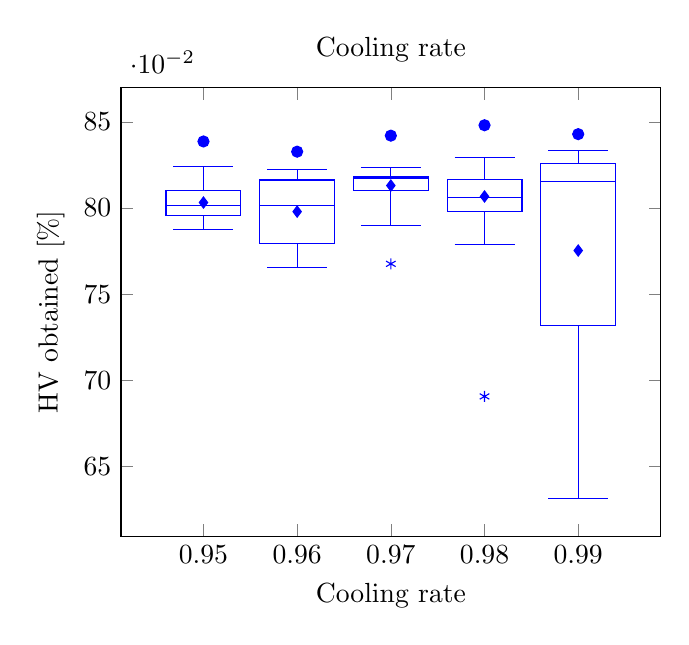
\begin{tikzpicture} 
\begin{axis}[ 
title={Cooling rate}, 
boxplot/draw direction=y, 
xtick={1,2,3,4,5}, 
xticklabels={0.95,0.96,0.97,0.98,0.99}, 
x tick label style={rotate=0, align=center}, 
xlabel={Cooling rate}, 
% y tick label style={/pgf/number format/.cd,fixed,precision=3, zerofill}, 
scaled y ticks={base 10:2}, 
ylabel={HV obtained [\%]}, 
] 

% ############## Cooling_rate=0.95 ################## 
\addplot[boxplot, mark=asterisk, 
boxplot prepared={ 
lower whisker=0.78756, 
upper whisker=0.82393, 
lower quartile=0.79544, 
upper quartile=0.81009, 
median=0.80145, 
average=0.8032}, 
color = blue, solid, area legend] 
coordinates {}; 
\addplot[only marks,mark=*,color = blue]coordinates{(1,0.83866)}; 

% ############## Cooling_rate=0.96 ################## 
\addplot[boxplot, mark=asterisk, 
boxplot prepared={ 
lower whisker=0.76531, 
upper whisker=0.8224, 
lower quartile=0.77953, 
upper quartile=0.81629, 
median=0.80137, 
average=0.7979}, 
color = blue, solid, area legend] 
coordinates {}; 
\addplot[only marks,mark=*,color = blue]coordinates{(2,0.83273)}; 

% ############## Cooling_rate=0.97 ################## 
\addplot[boxplot, mark=asterisk, 
boxplot prepared={ 
lower whisker=0.79008, 
upper whisker=0.82341, 
lower quartile=0.81016, 
upper quartile=0.818, 
median=0.81706, 
average=0.81304}, 
color = blue, solid, area legend] 
coordinates {
(3,0.7676)}; 
\addplot[only marks,mark=*,color = blue]coordinates{(3,0.84203)}; 

% ############## Cooling_rate=0.98 ################## 
\addplot[boxplot, mark=asterisk, 
boxplot prepared={ 
lower whisker=0.77879, 
upper whisker=0.82936, 
lower quartile=0.79797, 
upper quartile=0.81637, 
median=0.80634, 
average=0.80674}, 
color = blue, solid, area legend] 
coordinates {
(4,0.69061)}; 
\addplot[only marks,mark=*,color = blue]coordinates{(4,0.84808)}; 

% ############## Cooling_rate=0.99 ################## 
\addplot[boxplot, mark=asterisk, 
boxplot prepared={ 
lower whisker=0.63115, 
upper whisker=0.83351, 
lower quartile=0.73178, 
upper quartile=0.82599, 
median=0.81548, 
average=0.77534}, 
color = blue, solid, area legend] 
coordinates {}; 
\addplot[only marks,mark=*,color = blue]coordinates{(5,0.84291)}; 

\end{axis}
\end{tikzpicture}
\end{figure} 

% ######################## UTRP SA Maximum attempts ######################## 
\begin{figure} 
\centering 
\tikzsetnextfilename{UTRP_DBMOSA_BP_max_attempts} 
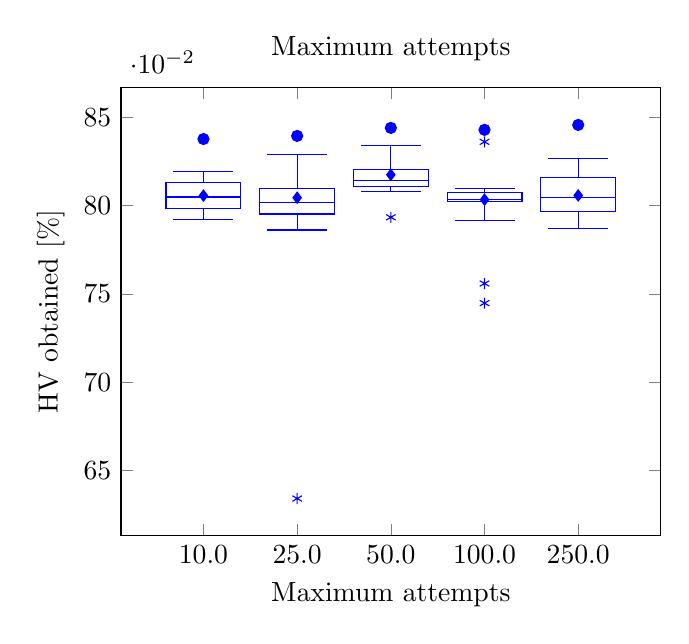
\begin{tikzpicture} 
\begin{axis}[ 
title={Maximum attempts}, 
boxplot/draw direction=y, 
xtick={1,2,3,4,5}, 
xticklabels={10.0,25.0,50.0,100.0,250.0}, 
x tick label style={rotate=0, align=center}, 
xlabel={Maximum attempts}, 
% y tick label style={/pgf/number format/.cd,fixed,precision=3, zerofill}, 
scaled y ticks={base 10:2}, 
ylabel={HV obtained [\%]}, 
] 

% ############## max_attempts=10.0 ################## 
\addplot[boxplot, mark=asterisk, 
boxplot prepared={ 
lower whisker=0.79218, 
upper whisker=0.81949, 
lower quartile=0.79834, 
upper quartile=0.81317, 
median=0.80489, 
average=0.80564}, 
color = blue, solid, area legend] 
coordinates {}; 
\addplot[only marks,mark=*,color = blue]coordinates{(1,0.83772)}; 

% ############## max_attempts=25.0 ################## 
\addplot[boxplot, mark=asterisk, 
boxplot prepared={ 
lower whisker=0.78621, 
upper whisker=0.82911, 
lower quartile=0.79524, 
upper quartile=0.80988, 
median=0.80164, 
average=0.80447}, 
color = blue, solid, area legend] 
coordinates {
(2,0.63407)}; 
\addplot[only marks,mark=*,color = blue]coordinates{(2,0.83949)}; 

% ############## max_attempts=50.0 ################## 
\addplot[boxplot, mark=asterisk, 
boxplot prepared={ 
lower whisker=0.80814, 
upper whisker=0.834, 
lower quartile=0.81063, 
upper quartile=0.82039, 
median=0.81411, 
average=0.81747}, 
color = blue, solid, area legend] 
coordinates {
(3,0.79337)}; 
\addplot[only marks,mark=*,color = blue]coordinates{(3,0.84402)}; 

% ############## max_attempts=100.0 ################## 
\addplot[boxplot, mark=asterisk, 
boxplot prepared={ 
lower whisker=0.79154, 
upper whisker=0.80968, 
lower quartile=0.80211, 
upper quartile=0.80746, 
median=0.80346, 
average=0.8034}, 
color = blue, solid, area legend] 
coordinates {
(4,0.83612)
(4,0.75587)
(4,0.74476)}; 
\addplot[only marks,mark=*,color = blue]coordinates{(4,0.84293)}; 

% ############## max_attempts=250.0 ################## 
\addplot[boxplot, mark=asterisk, 
boxplot prepared={ 
lower whisker=0.78687, 
upper whisker=0.82684, 
lower quartile=0.79646, 
upper quartile=0.81573, 
median=0.80474, 
average=0.80574}, 
color = blue, solid, area legend] 
coordinates {}; 
\addplot[only marks,mark=*,color = blue]coordinates{(5,0.84571)}; 

\end{axis}
\end{tikzpicture}
\end{figure} 

% ######################## UTRP SA Max iterations per epoch ######################## 
\begin{figure} 
\centering 
\tikzsetnextfilename{UTRP_DBMOSA_BP_max_iterations_per_epoch} 
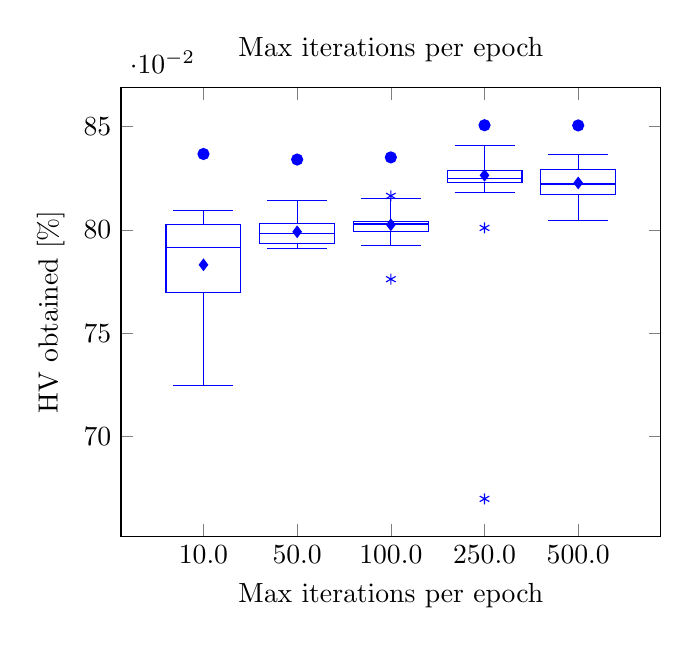
\begin{tikzpicture} 
\begin{axis}[ 
title={Max iterations per epoch}, 
boxplot/draw direction=y, 
xtick={1,2,3,4,5}, 
xticklabels={10.0,50.0,100.0,250.0,500.0}, 
x tick label style={rotate=0, align=center}, 
xlabel={Max iterations per epoch}, 
% y tick label style={/pgf/number format/.cd,fixed,precision=3, zerofill}, 
scaled y ticks={base 10:2}, 
ylabel={HV obtained [\%]}, 
] 

% ############## max_iterations_t=10.0 ################## 
\addplot[boxplot, mark=asterisk, 
boxplot prepared={ 
lower whisker=0.72471, 
upper whisker=0.80954, 
lower quartile=0.76966, 
upper quartile=0.80284, 
median=0.79136, 
average=0.78315}, 
color = blue, solid, area legend] 
coordinates {}; 
\addplot[only marks,mark=*,color = blue]coordinates{(1,0.8368)}; 

% ############## max_iterations_t=50.0 ################## 
\addplot[boxplot, mark=asterisk, 
boxplot prepared={ 
lower whisker=0.79087, 
upper whisker=0.81446, 
lower quartile=0.79326, 
upper quartile=0.80315, 
median=0.79821, 
average=0.79913}, 
color = blue, solid, area legend] 
coordinates {}; 
\addplot[only marks,mark=*,color = blue]coordinates{(2,0.83411)}; 

% ############## max_iterations_t=100.0 ################## 
\addplot[boxplot, mark=asterisk, 
boxplot prepared={ 
lower whisker=0.79264, 
upper whisker=0.81521, 
lower quartile=0.7993, 
upper quartile=0.80412, 
median=0.80289, 
average=0.80251}, 
color = blue, solid, area legend] 
coordinates {
(3,0.81651)
(3,0.77618)}; 
\addplot[only marks,mark=*,color = blue]coordinates{(3,0.83515)}; 

% ############## max_iterations_t=250.0 ################## 
\addplot[boxplot, mark=asterisk, 
boxplot prepared={ 
lower whisker=0.81819, 
upper whisker=0.84073, 
lower quartile=0.82278, 
upper quartile=0.82897, 
median=0.82495, 
average=0.8265}, 
color = blue, solid, area legend] 
coordinates {
(4,0.66983)
(4,0.80101)}; 
\addplot[only marks,mark=*,color = blue]coordinates{(4,0.85072)}; 

% ############## max_iterations_t=500.0 ################## 
\addplot[boxplot, mark=asterisk, 
boxplot prepared={ 
lower whisker=0.80477, 
upper whisker=0.83656, 
lower quartile=0.81725, 
upper quartile=0.82944, 
median=0.82228, 
average=0.82276}, 
color = blue, solid, area legend] 
coordinates {}; 
\addplot[only marks,mark=*,color = blue]coordinates{(5,0.85062)}; 

\end{axis}
\end{tikzpicture}
\end{figure} 

% ######################## UTRP SA Maximum poor epochs ######################## 
\begin{figure} 
\centering 
\tikzsetnextfilename{UTRP_DBMOSA_BP_max_poor_epochs} 
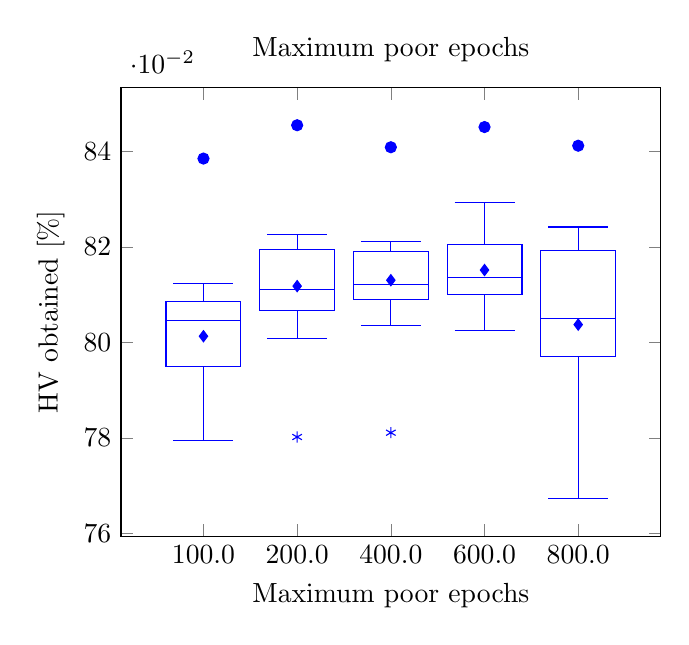
\begin{tikzpicture} 
\begin{axis}[ 
title={Maximum poor epochs}, 
boxplot/draw direction=y, 
xtick={1,2,3,4,5}, 
xticklabels={100.0,200.0,400.0,600.0,800.0}, 
x tick label style={rotate=0, align=center}, 
xlabel={Maximum poor epochs}, 
% y tick label style={/pgf/number format/.cd,fixed,precision=3, zerofill}, 
scaled y ticks={base 10:2}, 
ylabel={HV obtained [\%]}, 
] 

% ############## max_poor_epochs=100.0 ################## 
\addplot[boxplot, mark=asterisk, 
boxplot prepared={ 
lower whisker=0.77946, 
upper whisker=0.81233, 
lower quartile=0.79503, 
upper quartile=0.80856, 
median=0.80459, 
average=0.80131}, 
color = blue, solid, area legend] 
coordinates {}; 
\addplot[only marks,mark=*,color = blue]coordinates{(1,0.83852)}; 

% ############## max_poor_epochs=200.0 ################## 
\addplot[boxplot, mark=asterisk, 
boxplot prepared={ 
lower whisker=0.80086, 
upper whisker=0.82269, 
lower quartile=0.80678, 
upper quartile=0.81945, 
median=0.81113, 
average=0.81181}, 
color = blue, solid, area legend] 
coordinates {
(2,0.78021)}; 
\addplot[only marks,mark=*,color = blue]coordinates{(2,0.8455)}; 

% ############## max_poor_epochs=400.0 ################## 
\addplot[boxplot, mark=asterisk, 
boxplot prepared={ 
lower whisker=0.80351, 
upper whisker=0.82111, 
lower quartile=0.80896, 
upper quartile=0.81902, 
median=0.81211, 
average=0.81304}, 
color = blue, solid, area legend] 
coordinates {
(3,0.78111)}; 
\addplot[only marks,mark=*,color = blue]coordinates{(3,0.84089)}; 

% ############## max_poor_epochs=600.0 ################## 
\addplot[boxplot, mark=asterisk, 
boxplot prepared={ 
lower whisker=0.80247, 
upper whisker=0.82926, 
lower quartile=0.81014, 
upper quartile=0.82061, 
median=0.81366, 
average=0.81518}, 
color = blue, solid, area legend] 
coordinates {}; 
\addplot[only marks,mark=*,color = blue]coordinates{(4,0.84512)}; 

% ############## max_poor_epochs=800.0 ################## 
\addplot[boxplot, mark=asterisk, 
boxplot prepared={ 
lower whisker=0.76726, 
upper whisker=0.82418, 
lower quartile=0.79705, 
upper quartile=0.81928, 
median=0.80499, 
average=0.80375}, 
color = blue, solid, area legend] 
coordinates {}; 
\addplot[only marks,mark=*,color = blue]coordinates{(5,0.84121)}; 

\end{axis}
\end{tikzpicture}
\end{figure} 

% ######################## UTRP SA Maximum reheating times ######################## 
\begin{figure} 
\centering 
\tikzsetnextfilename{UTRP_DBMOSA_BP_max_reheating_times} 
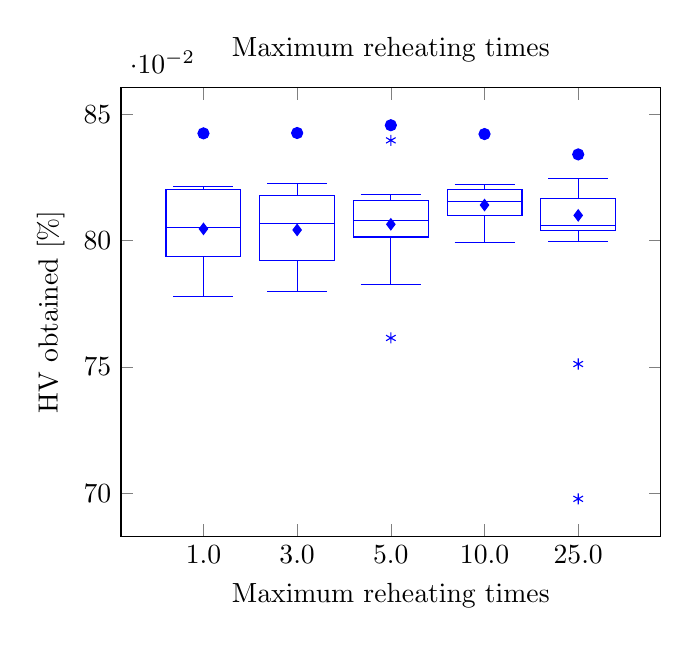
\begin{tikzpicture} 
\begin{axis}[ 
title={Maximum reheating times}, 
boxplot/draw direction=y, 
xtick={1,2,3,4,5}, 
xticklabels={1.0,3.0,5.0,10.0,25.0}, 
x tick label style={rotate=0, align=center}, 
xlabel={Maximum reheating times}, 
% y tick label style={/pgf/number format/.cd,fixed,precision=3, zerofill}, 
scaled y ticks={base 10:2}, 
ylabel={HV obtained [\%]}, 
] 

% ############## max_reheating_times=1.0 ################## 
\addplot[boxplot, mark=asterisk, 
boxplot prepared={ 
lower whisker=0.77802, 
upper whisker=0.82144, 
lower quartile=0.79363, 
upper quartile=0.82025, 
median=0.80502, 
average=0.80462}, 
color = blue, solid, area legend] 
coordinates {}; 
\addplot[only marks,mark=*,color = blue]coordinates{(1,0.84243)}; 

% ############## max_reheating_times=3.0 ################## 
\addplot[boxplot, mark=asterisk, 
boxplot prepared={ 
lower whisker=0.7799, 
upper whisker=0.82252, 
lower quartile=0.79199, 
upper quartile=0.81796, 
median=0.80687, 
average=0.8042}, 
color = blue, solid, area legend] 
coordinates {}; 
\addplot[only marks,mark=*,color = blue]coordinates{(2,0.84258)}; 

% ############## max_reheating_times=5.0 ################## 
\addplot[boxplot, mark=asterisk, 
boxplot prepared={ 
lower whisker=0.78258, 
upper whisker=0.81814, 
lower quartile=0.80141, 
upper quartile=0.81579, 
median=0.80778, 
average=0.80643}, 
color = blue, solid, area legend] 
coordinates {
(3,0.83966)
(3,0.76143)}; 
\addplot[only marks,mark=*,color = blue]coordinates{(3,0.84565)}; 

% ############## max_reheating_times=10.0 ################## 
\addplot[boxplot, mark=asterisk, 
boxplot prepared={ 
lower whisker=0.79939, 
upper whisker=0.82212, 
lower quartile=0.81002, 
upper quartile=0.82004, 
median=0.81549, 
average=0.81405}, 
color = blue, solid, area legend] 
coordinates {}; 
\addplot[only marks,mark=*,color = blue]coordinates{(4,0.84216)}; 

% ############## max_reheating_times=25.0 ################## 
\addplot[boxplot, mark=asterisk, 
boxplot prepared={ 
lower whisker=0.79964, 
upper whisker=0.82469, 
lower quartile=0.80392, 
upper quartile=0.81649, 
median=0.80588, 
average=0.80996}, 
color = blue, solid, area legend] 
coordinates {
(5,0.75112)
(5,0.69774)}; 
\addplot[only marks,mark=*,color = blue]coordinates{(5,0.8341)}; 

\end{axis}
\end{tikzpicture}
\end{figure} 

% ######################## UTRP SA Minimum accepts ######################## 
\begin{figure} 
\centering 
\tikzsetnextfilename{UTRP_DBMOSA_BP_min_accepts} 
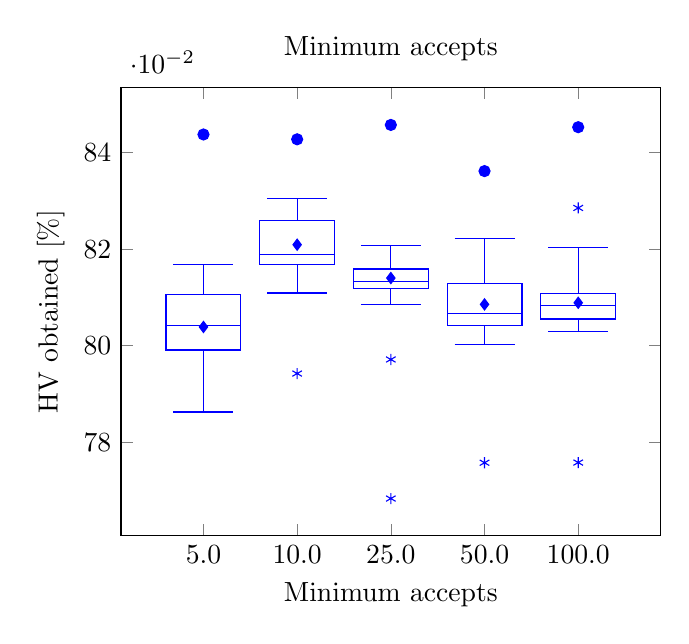
\begin{tikzpicture} 
\begin{axis}[ 
title={Minimum accepts}, 
boxplot/draw direction=y, 
xtick={1,2,3,4,5}, 
xticklabels={5.0,10.0,25.0,50.0,100.0}, 
x tick label style={rotate=0, align=center}, 
xlabel={Minimum accepts}, 
% y tick label style={/pgf/number format/.cd,fixed,precision=3, zerofill}, 
scaled y ticks={base 10:2}, 
ylabel={HV obtained [\%]}, 
] 

% ############## min_accepts=5.0 ################## 
\addplot[boxplot, mark=asterisk, 
boxplot prepared={ 
lower whisker=0.78623, 
upper whisker=0.81687, 
lower quartile=0.79909, 
upper quartile=0.81059, 
median=0.80411, 
average=0.80387}, 
color = blue, solid, area legend] 
coordinates {}; 
\addplot[only marks,mark=*,color = blue]coordinates{(1,0.84376)}; 

% ############## min_accepts=10.0 ################## 
\addplot[boxplot, mark=asterisk, 
boxplot prepared={ 
lower whisker=0.8109, 
upper whisker=0.8305, 
lower quartile=0.81686, 
upper quartile=0.82587, 
median=0.81893, 
average=0.82092}, 
color = blue, solid, area legend] 
coordinates {
(2,0.79421)}; 
\addplot[only marks,mark=*,color = blue]coordinates{(2,0.84276)}; 

% ############## min_accepts=25.0 ################## 
\addplot[boxplot, mark=asterisk, 
boxplot prepared={ 
lower whisker=0.80844, 
upper whisker=0.82081, 
lower quartile=0.8119, 
upper quartile=0.81587, 
median=0.81325, 
average=0.81401}, 
color = blue, solid, area legend] 
coordinates {
(3,0.79712)
(3,0.7683)}; 
\addplot[only marks,mark=*,color = blue]coordinates{(3,0.84574)}; 

% ############## min_accepts=50.0 ################## 
\addplot[boxplot, mark=asterisk, 
boxplot prepared={ 
lower whisker=0.80031, 
upper whisker=0.82218, 
lower quartile=0.80412, 
upper quartile=0.81288, 
median=0.80667, 
average=0.80854}, 
color = blue, solid, area legend] 
coordinates {
(4,0.77572)}; 
\addplot[only marks,mark=*,color = blue]coordinates{(4,0.83617)}; 

% ############## min_accepts=100.0 ################## 
\addplot[boxplot, mark=asterisk, 
boxplot prepared={ 
lower whisker=0.80291, 
upper whisker=0.8204, 
lower quartile=0.80552, 
upper quartile=0.81075, 
median=0.80828, 
average=0.80888}, 
color = blue, solid, area legend] 
coordinates {
(5,0.77576)
(5,0.82853)}; 
\addplot[only marks,mark=*,color = blue]coordinates{(5,0.84527)}; 

\end{axis}
\end{tikzpicture}
\end{figure} 

% ######################## UTRP SA Reheating rate ######################## 
\begin{figure} 
\centering 
\tikzsetnextfilename{UTRP_DBMOSA_BP_reheating_rate} 
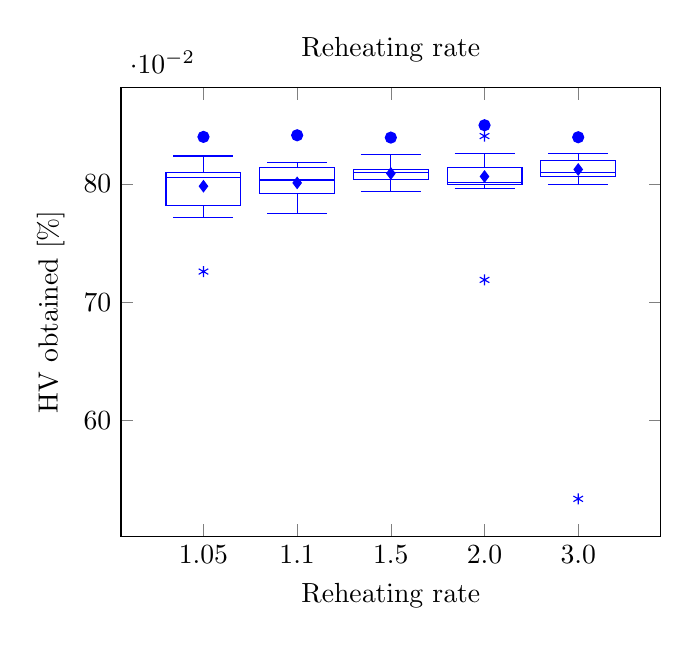
\begin{tikzpicture} 
\begin{axis}[ 
title={Reheating rate}, 
boxplot/draw direction=y, 
xtick={1,2,3,4,5}, 
xticklabels={1.05,1.1,1.5,2.0,3.0}, 
x tick label style={rotate=0, align=center}, 
xlabel={Reheating rate}, 
% y tick label style={/pgf/number format/.cd,fixed,precision=3, zerofill}, 
scaled y ticks={base 10:2}, 
ylabel={HV obtained [\%]}, 
] 

% ############## Reheating_rate=1.05 ################## 
\addplot[boxplot, mark=asterisk, 
boxplot prepared={ 
lower whisker=0.77182, 
upper whisker=0.8236, 
lower quartile=0.78147, 
upper quartile=0.80971, 
median=0.80545, 
average=0.79809}, 
color = blue, solid, area legend] 
coordinates {
(1,0.7259)}; 
\addplot[only marks,mark=*,color = blue]coordinates{(1,0.83981)}; 

% ############## Reheating_rate=1.1 ################## 
\addplot[boxplot, mark=asterisk, 
boxplot prepared={ 
lower whisker=0.77513, 
upper whisker=0.81824, 
lower quartile=0.79181, 
upper quartile=0.81424, 
median=0.80331, 
average=0.80091}, 
color = blue, solid, area legend] 
coordinates {}; 
\addplot[only marks,mark=*,color = blue]coordinates{(2,0.84117)}; 

% ############## Reheating_rate=1.5 ################## 
\addplot[boxplot, mark=asterisk, 
boxplot prepared={ 
lower whisker=0.79346, 
upper whisker=0.8249, 
lower quartile=0.80356, 
upper quartile=0.81246, 
median=0.80995, 
average=0.80885}, 
color = blue, solid, area legend] 
coordinates {}; 
\addplot[only marks,mark=*,color = blue]coordinates{(3,0.8392)}; 

% ############## Reheating_rate=2.0 ################## 
\addplot[boxplot, mark=asterisk, 
boxplot prepared={ 
lower whisker=0.79602, 
upper whisker=0.82604, 
lower quartile=0.79986, 
upper quartile=0.81363, 
median=0.80147, 
average=0.80633}, 
color = blue, solid, area legend] 
coordinates {
(4,0.71888)
(4,0.8405)}; 
\addplot[only marks,mark=*,color = blue]coordinates{(4,0.84965)}; 

% ############## Reheating_rate=3.0 ################## 
\addplot[boxplot, mark=asterisk, 
boxplot prepared={ 
lower whisker=0.79933, 
upper whisker=0.82576, 
lower quartile=0.80664, 
upper quartile=0.81968, 
median=0.80967, 
average=0.81223}, 
color = blue, solid, area legend] 
coordinates {
(5,0.5337)}; 
\addplot[only marks,mark=*,color = blue]coordinates{(5,0.8395)}; 

\end{axis}
\end{tikzpicture}
\end{figure} 

% ######################## UTRP SA Starting temperature ######################## 
\begin{figure} 
\centering 
\tikzsetnextfilename{UTRP_DBMOSA_BP_initial_temp} 
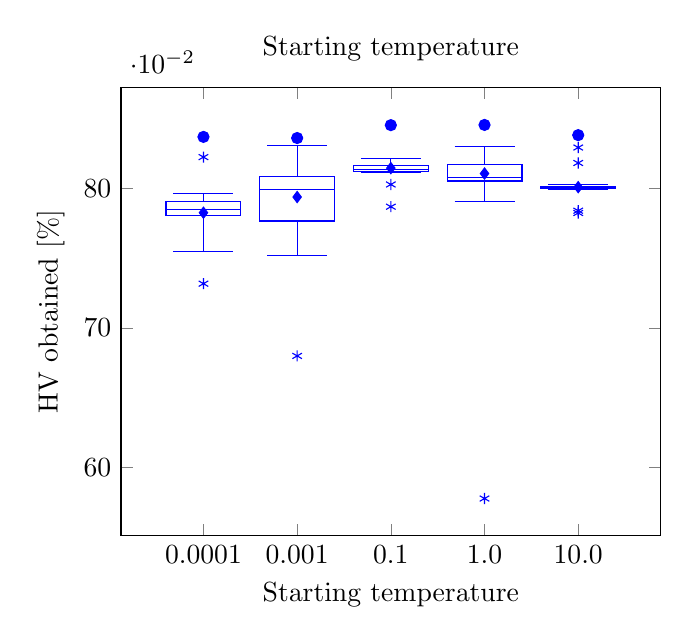
\begin{tikzpicture} 
\begin{axis}[ 
title={Starting temperature}, 
boxplot/draw direction=y, 
xtick={1,2,3,4,5}, 
xticklabels={0.0001,0.001,0.1,1.0,10.0}, 
x tick label style={rotate=0, align=center}, 
xlabel={Starting temperature}, 
% y tick label style={/pgf/number format/.cd,fixed,precision=3, zerofill}, 
scaled y ticks={base 10:2}, 
ylabel={HV obtained [\%]}, 
] 

% ############## Temp=0.0001 ################## 
\addplot[boxplot, mark=asterisk, 
boxplot prepared={ 
lower whisker=0.75446, 
upper whisker=0.79632, 
lower quartile=0.78021, 
upper quartile=0.79074, 
median=0.78483, 
average=0.78248}, 
color = blue, solid, area legend] 
coordinates {
(1,0.7317)
(1,0.82229)}; 
\addplot[only marks,mark=*,color = blue]coordinates{(1,0.83676)}; 

% ############## Temp=0.001 ################## 
\addplot[boxplot, mark=asterisk, 
boxplot prepared={ 
lower whisker=0.75208, 
upper whisker=0.83077, 
lower quartile=0.77653, 
upper quartile=0.8082, 
median=0.79891, 
average=0.79373}, 
color = blue, solid, area legend] 
coordinates {
(2,0.68)}; 
\addplot[only marks,mark=*,color = blue]coordinates{(2,0.83594)}; 

% ############## Temp=0.1 ################## 
\addplot[boxplot, mark=asterisk, 
boxplot prepared={ 
lower whisker=0.81111, 
upper whisker=0.82124, 
lower quartile=0.81197, 
upper quartile=0.81607, 
median=0.81338, 
average=0.81439}, 
color = blue, solid, area legend] 
coordinates {
(3,0.80269)
(3,0.78679)}; 
\addplot[only marks,mark=*,color = blue]coordinates{(3,0.84516)}; 

% ############## Temp=1.0 ################## 
\addplot[boxplot, mark=asterisk, 
boxplot prepared={ 
lower whisker=0.79027, 
upper whisker=0.82959, 
lower quartile=0.80517, 
upper quartile=0.81696, 
median=0.80785, 
average=0.81052}, 
color = blue, solid, area legend] 
coordinates {
(4,0.57793)}; 
\addplot[only marks,mark=*,color = blue]coordinates{(4,0.84532)}; 

% ############## Temp=10.0 ################## 
\addplot[boxplot, mark=asterisk, 
boxplot prepared={ 
lower whisker=0.79948, 
upper whisker=0.80272, 
lower quartile=0.79998, 
upper quartile=0.80136, 
median=0.80053, 
average=0.80078}, 
color = blue, solid, area legend] 
coordinates {
(5,0.81808)
(5,0.7823)
(5,0.78392)
(5,0.82915)}; 
\addplot[only marks,mark=*,color = blue]coordinates{(5,0.83802)}; 

\end{axis}
\end{tikzpicture}
\end{figure} 
\begin{table}
\centering
\caption{Legend for the boxplot.}
\begin{tabular}{ll}
\toprule
 Index &  Name \\
\midrule
     0 &    10 \\
     1 &    50 \\
     2 &   100 \\
     3 &   250 \\
     4 &   500 \\
\bottomrule
\end{tabular}
\end{table}

\end{document}
